\documentclass{beamer}
\usepackage[croatian]{babel}
\usepackage[utf8]{inputenc}
\usepackage{beamerthemeBerlin}
\usepackage{graphicx}
\usepackage{verbatim}
\usepackage{hyperref}
\begin{document}

\title{Markdown}
\author{Deni Klen, Fran Grenko i Mihael Petranović}
\institute{Tehnički fakultet Rijeka, Sveučilište u Rijeci}
\maketitle






\begin{frame}
	\frametitle{Što je Markdown?}

 	\begin{minipage}[0.2\textheight]{\textwidth}
 	\begin{columns}[T]
 	\begin{column}{0.8\textwidth}
 	\begin{itemize}
		\item{Markdown je lagani markup jezik sa sintaksom za oblikovanje običnog teksta čija je glavna značajka lako čitanje i pisanje (easy-to-read i easy-to-write)}
		\item{Stvorili su ga John Gruber i Aaron Swartz 2004. godine}
		\item{Postoji više inačica koje se i dalje razvijaju \\ npr. \textit{CommonMark, GFM, Markdown Extra} ...}
		\item{Najčešće se koristi za formatiranje "README" datoteka}
	\end{itemize}
	\end{column}
	\begin{column}{0.2\textwidth}
	
\includegraphics[width=2.5cm]{Slike/markdown.png}
	\end{column}
	\end{columns}
	\end{minipage}

\end{frame}





\begin{frame}
	\frametitle{Upotreba Markdown-a}

 	\begin{minipage}[0.2\textheight]{\textwidth}
 	\begin{columns}[T]
 	\begin{column}{0.8\textwidth}
 	\begin{itemize}
		\item{Osnovna upotreba je formatiranje, pisanje i uređivanje različiti tekstualnih datoteka, uljepšavanje teksta itd.}
		\item{\textit{*Ukošavanje*}, \textbf{**podebljavanje**}, \emph{isticanje} i \underline{podcrtavanje} teksta neke su od mogućnosti uljepšavanja teksta u MarkDownu}
		\item{Markdown također omogućuje kreiranje zaglavlja i lista te ubacivanje poveznica, slika i citata}
	\end{itemize}
	\end{column}
	\end{columns}
	\end{minipage}

\end{frame}

\begin{frame}[fragile]
	\frametitle{Primjer sintakse}

	\begin{verbatim}
	# Markdown
	Uz pomoć markdown-a možemo vrlo lako **podebljati** ,
	 *ukositi* i _podcrtati_ tekst.
	\end{verbatim}

	\begin{figure}[b]
		\caption{Ispis teksta}
		
\includegraphics[width = 0.8\linewidth]{Slike/kod.png}
		
	\end{figure}
\end{frame}

\begin{frame}[fragile]
	\frametitle{Primjer sintakse}
	
	\begin{verbatim}
	Lagano se mogu kreirati [linkovi](www.google.com)
	i slike  ![slika](macak.jpg)

	\end{verbatim}

	\begin{figure}[b]
	\caption{Ispis linkova i slika}
	
\includegraphics[width = 0.8\linewidth]{Slike/kod2.png}
	\end{figure}

\end{frame}





\begin{frame}
	\frametitle{CommonMark}

 	\begin{minipage}[0.2\textheight]{\textwidth}
 	\begin{columns}[T]
 	\begin{column}{0.8\textwidth}
 	\begin{itemize}
		\item{Jedna od najpopularnijih inačica prvotnog Markdown jezika}
		\item{Želja developera CommonMark-a je stvorit jedinstveni oblik Markdown sintakse koju bi svi mogli koristiti kako ne bi dolazilo do razlika u prikazivanju \\(razlike se događaju jer se tekst drugačije "čita" i prikazuje za različite inačice Markdown sintaksa)}
	\end{itemize}
	\end{column}
	\end{columns}
	\end{minipage}

\end{frame}

\begin{frame}
	\frametitle{Markdown - CommonMark razlike}

 	\begin{minipage}[0.2\textheight]{\textwidth}
 	\begin{columns}[T]
 	\begin{column}{0.8\textwidth}
 	\begin{itemize}
 		\item{Linkovi
 		\begin{itemize}
 			\item{Markdown: [link](url sa razmacima)}
 			\item{CommonMark: [link](url\%20sa\%razmacima)}
 		\end{itemize}}
 		\item{Liste
 		\begin{itemize}
 			\item{U Markdown-u dva razmaka - paragraf}
 			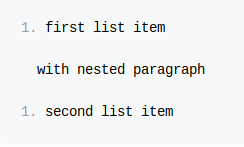
\includegraphics[width=4cm, height=1.5cm]{Slike/Usporedba1.png}
 			\item{U CommonMarku-u četiri razmaka - paragraf}
 			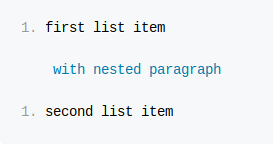
\includegraphics[width=4cm,  height=1.5cm]{Slike/usporeda2.png}
 		\end{itemize}}
	\end{itemize}
	\end{column}
	\end{columns}
	\end{minipage}

\end{frame}

\begin{frame}
	\frametitle{Markdown - CommonMark razlike}

 	\begin{minipage}[0.2\textheight]{\textwidth}
 	\begin{columns}[T]
 	\begin{column}{0.8\textwidth}
 	\begin{itemize}
 		\item{Naslovi
 		\begin{itemize}
 			\item{Markdown: \# Naslov}
 			\item{CommonMark: \textbackslash \# Naslov}
 		\end{itemize}}
 		\item{Tablice
 		\begin{itemize}
 			\item{U Markdown-u dostupne u bilo kojoj formi}
 			\item{U CommonMarku-u dostupne u HTML formi te dostupne u vise oblika}
 		\end{itemize}}
	\end{itemize}
	\end{column}
	\end{columns}
	\end{minipage}

\end{frame}





\begin{frame}
	\frametitle{GFM - GitHub Flavored Markdown}

 	\begin{minipage}[0.2\textheight]{\textwidth}
 	\begin{columns}[T]
 	\begin{column}{0.8\textwidth}
 	\begin{itemize}
		\item{Inačica koja se bazira ponajviše na CommonMark specifikacijama}
		\item{Koristi se na stranicama GitHub Enterprise i \href{https://github.com/}{GitHub.com}}
	\end{itemize}
	\end{column}
	\begin{column}{0.2\textwidth}
	
\includegraphics[width=2.5cm]{Slike/githublogo.png}
	\end{column}
	\end{columns}
	\end{minipage}

\end{frame}


\begin{frame}
	\frametitle{GFM - GitHub Flavored Markdown}

	Za razliku od CommonMark-a sadrži:
	\begin{itemize}
		\item{Tablice}
		\item{Precrtani tekst}
		\item{Autolinkove}
		\item{Task liste}
	\end{itemize}
\end{frame}

\begin{frame}[fragile]
	\frametitle{GFM - GitHub Flavored Markdown - sintaksa}

	\textbf{Primjer precrtanog teksta:}

	\begin{verbatim}
	~~ This was mistaken text ~~
	\end{verbatim}

	\begin{figure}[htbp]
	
\includegraphics[width=0.3\textwidth]{Slike/kod3.png}
	
	\end{figure}

\end{frame}

\begin{frame}[fragile]
	\frametitle{GFM - GitHub Flavored Markdown - sintaksa}

	\textbf{Primjer task liste}

	\begin{verbatim}
	- [ ] Watch Breaking Bad
	- [ ] Finish this demo
	- [x] Fix all the things
	- [x] Be awesome
	\end{verbatim}

	\begin{figure}[htbp]
	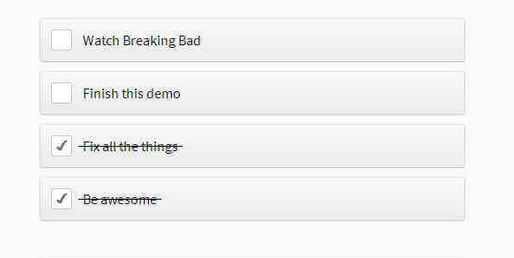
\includegraphics[width=0.6\textwidth]{Slike/kod4.png}
	
	\end{figure}
\end{frame}



\begin{frame}
	\frametitle{Markdown Extra}

 	\begin{minipage}[0.2\textheight]{\textwidth}
 	\begin{columns}[T]
 	\begin{column}{0.8\textwidth}
 	\begin{itemize}
 		\item{Ekstenzija PHP Markdown-a}
		\item{Omogućuje upotrebu značajki koje se nisu mogle upotrebljavati u prvotnoj Markdown sintaksi}
		\item{Primjeri: 
		\begin{itemize}
			\item{Markdown unutar HTML blokova}
			\item{Fusnote}
			\item{Liste definicija}
			\item{Tablice}
			\item{Skraćenice}...
		\end{itemize}}
	\end{itemize}
	\end{column}
	\end{columns}
	\end{minipage}

\end{frame}

\begin{frame}[fragile]
\frametitle{Markdown Extra - sintaksa}

\textbf{Primjer tablice:}
\begin{figure}[htbp]
	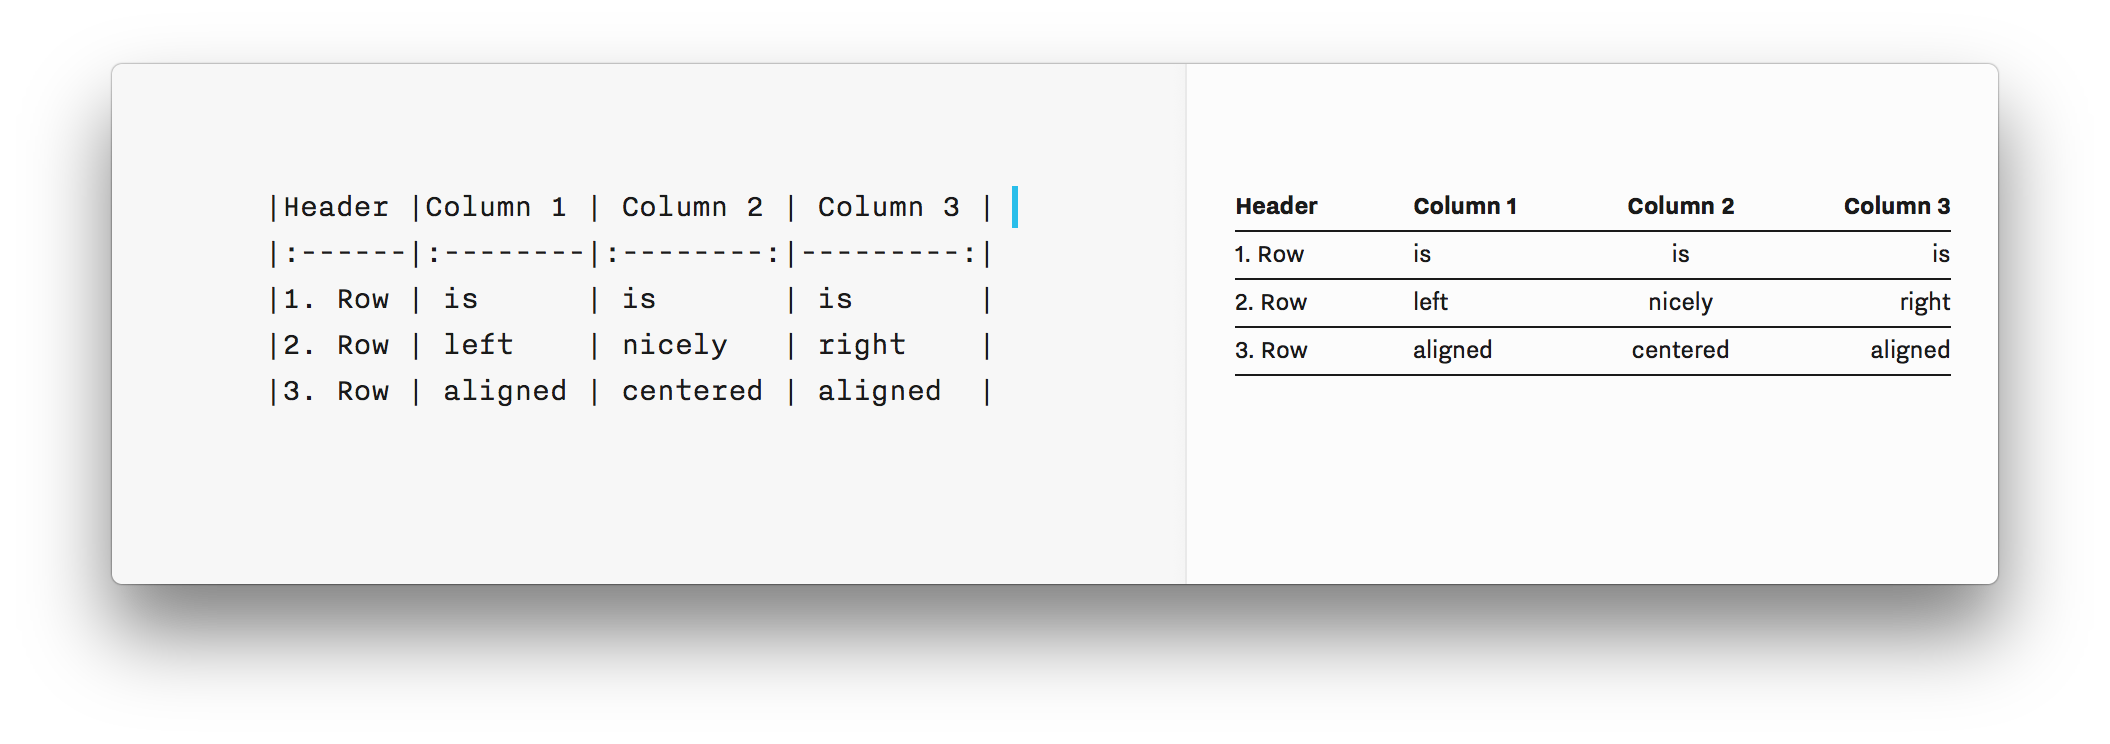
\includegraphics[width=1.1\textwidth]{Slike/table.png}
	
	\end{figure}


\end{frame}



\begin{frame}
	\frametitle{Literatura}

 	\begin{minipage}[0.2\textheight]{\textwidth}
 	\begin{columns}[T]
 	\begin{column}{0.8\textwidth}
 	\begin{itemize}
 		\item{Literatura:
 		\begin{itemize}
 			\item{\url{https://en.wikipedia.org/wiki/Markdown}}
 			\item{\url{https://www.markdowntutorial.com/}}
 			\item{\url{https://commonmark.org/help/}}
 			\item{\url{https://www.markdownguide.org/}}
 			\item{\url{https://github.github.com/gfm/}}
 			\item{\url{https://michelf.ca/projects/php-markdown/extra/}}
 		\end{itemize}}
	\end{itemize}
	\end{column}
	\end{columns}
	\end{minipage}

\end{frame}



\end{document}
